\label{ch:implementation}

Besides the realization of EDA sensors results relatively simple when compared with the circuitry of other devices, its limited diffusion at present implies a series of issues that are required to be addressed. More specifically:

\begin{itemize}
    \item EDA wearables oriented to research purposes tend to be \textbf{particularly expensive} (and most of the time unaffordable for small research projects)
    \item Well-known devices implementing EDA-related features do not provide Application Programming Interfaces for developers and do not provide open-source solutions either
\end{itemize}

The following chapter describes the implementation of a \textbf{simple} and completely \textbf{open-source} wearable device, aimed at providing a low-cost framework for the Electrodermal Activity measurement in \textbf{experimental contexts}.

\section{BITalino Electrodermal Activity Sensor}\label{sec:bitalino}

The sensor unit employed is the purpose-built \textbf{Electrodermal Activity Sensor} by \textbf{BITalino}. This constitutes a single module aimed at composing, along with many others sold by the company, the \textbf{BITalino (r)evolution Board Kit} \cite{bitalino-general}, an all-in-one device implementing a custom firmware for the collection and aggregation of data retrieved from bio-signals. Besides all the features implemented by these boards result interesting in research contexts, the main drawbacks are related to the \textbf{lack of mobility} that the device would cause, which is a primary concern within the bounds of fall detection systems.

Moreover, during the recent years the BITalino EDA module has been employed in a multitude of scientific publications which, overall, have proven that the device allows to reach optimal results in terms of cost-effective Electrodermal Activity analysis.

A \textbf{single EDA module} was purchased for a 25,00 € (Tax Excluded) price and a minimal \textbf{Arduino-based firmware} was implemented in order to retrieve measurements from the individual unit without having to rely on third-party solutions.

\subsection{Description and Features}\label{subsec:bitalino-features}

The EDA sensor module consists of a breakout board whose dimensions correspond to 12mm x 27mm \cite{bitalino-general}. A complete list of informations regarding the configuration of the unit is reported in Table \ref{toc:bitalino-features} .

\begin{table}[H]
\centering
\begin{tabular}{ll}
    \hline
    Parameter               & Value \\
    \hline
    Current                 & DC \\
    Range                   & 0-30 $\mu S$ \\
    Consumption             & $\pm 0.1 mA$ \\
    Bandwidth               & 0 - 2.8 Hz \\
    Measurement             & continuous \\
    Input Voltage Range     & 1.8 - 5.5 V \\
    \hline
\end{tabular}
\caption{Characteristics of the BITalino EDA sensor unit}
\label{toc:bitalino-features}
\end{table}

Furthermore, the device is sold in the three following configurations, according to the requirements of the customers: 
\begin{itemize}
    \item \textbf{Self-assemble}
    \item \textbf{Self-assemble} with \textbf{UC-E6 connectors}
    \item \textbf{Assembled}
\end{itemize}

\vspace{3mm}

The first version consists of the breakout board only and requires manual soldering to obtain a complete configuration. The second one provides, instead, pre-installed UC-E6 connectors in order to facilitate the connection to a BITalino board by using apposite homonymous cables. The assembled version is, lastly, presented as a ready-made configuration that includes: 

\begin{itemize}
    \item Pre-soldered electrodes
    \item Pre-soldered UC-E6 cable
    \item A 3D printed ABS case containing the breakout board
\end{itemize}

% https://bitalino.com/storage/uploads/media/homeguide4-eda.pdf

\subsection{Modifications applied}\label{subsec:bitalno-modifications}

In order to exploit the convenience provided by the case and the pre-soldered electrodes, an \textbf{assembled unit} was acquired and subsequently \textbf{modified} in order to implement the connection with a third-party microcontroller. More specifically, the modification procedure consisted of the following steps: 

\begin{enumerate}
    \item Opening of the ABS case
    \item Desoldering the four UC-E6 connector cables from their respective pins on the breakout board
    \item Soldering a dupont cable on each one of the pins
    \item Widening the cable conduit of the ABS case in order to allow the passage of the previously soldered cables
    \item Closing back the ABS case
\end{enumerate}

The role of the pins provided by the breakout board is depicted by the diagram reported in figure \ref{fig:bitalino-pinmap}

\begin{figure}[h]
    \centering
    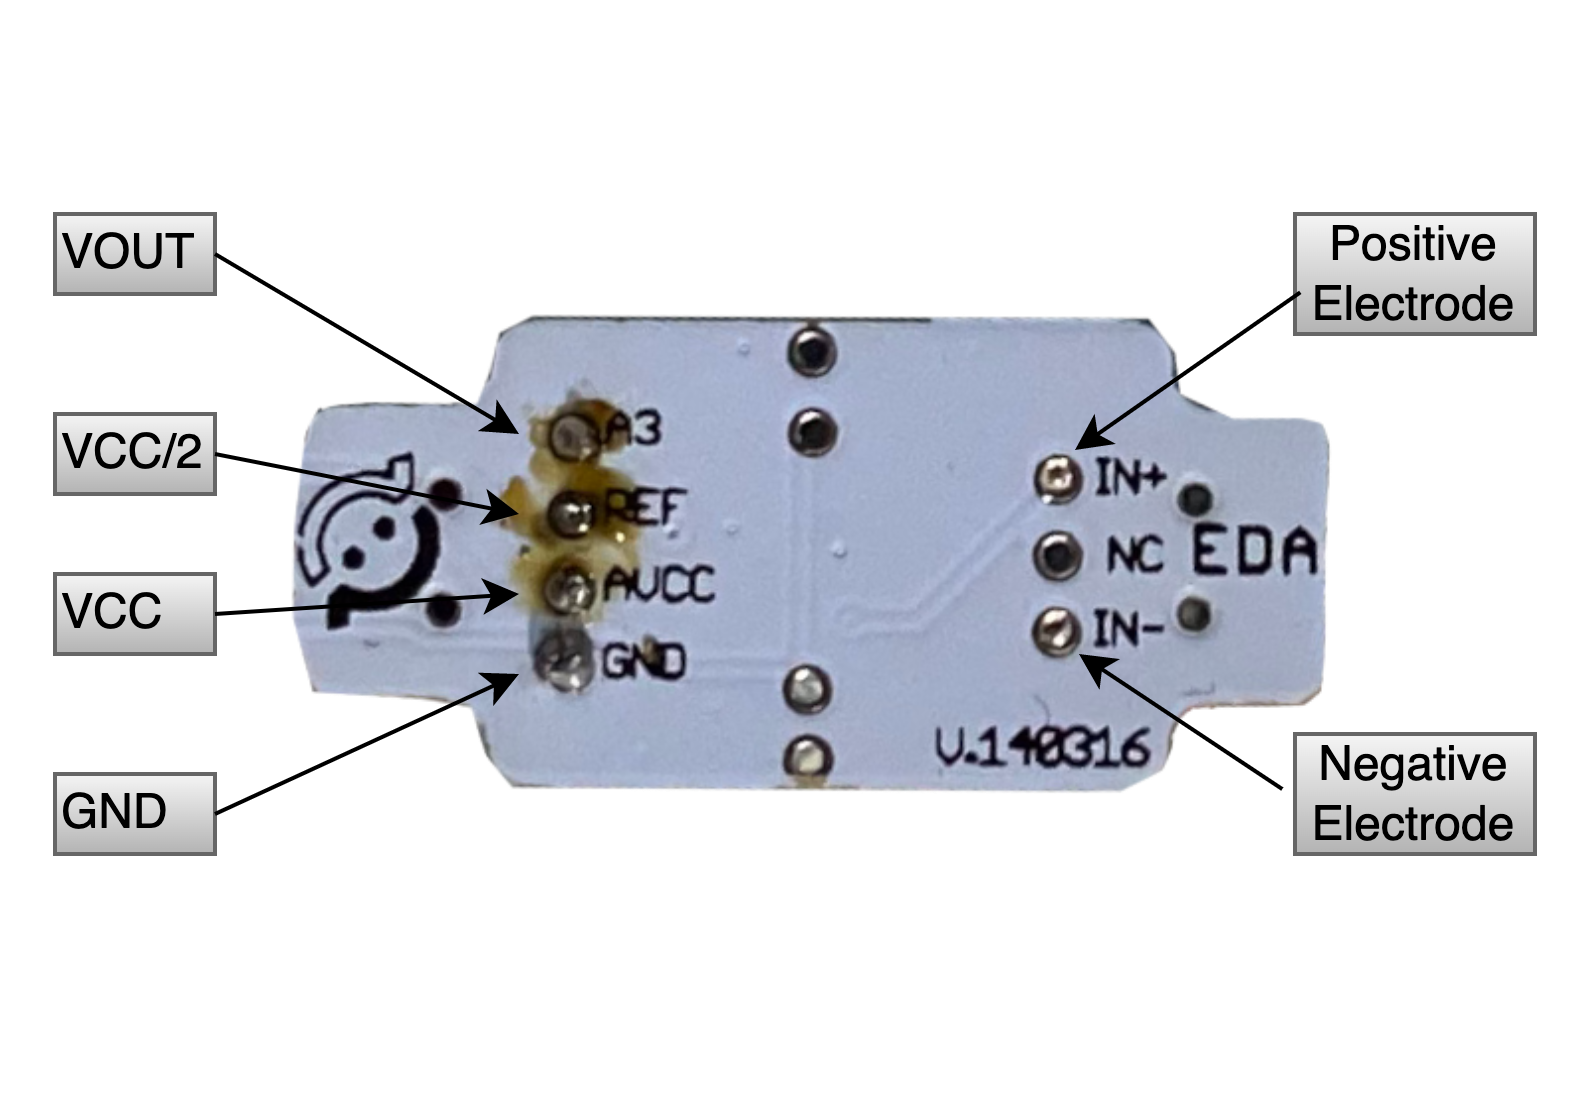
\includegraphics[width=10cm]{./images/bitalino.drawio.png}
    \caption{BITalino EDA sensor pin mapping}
    \label{fig:bitalino-pinmap}
\end{figure}

\vspace{1cm}

More specifically, the function of each pin is reported in table \ref{toc:bitalino-pinmap-table}

\begin{table}[H]
\centering
\begin{tabular}{ll}
    \hline
    \textbf{Pin}            & \textbf{Application} \\
    \hline
    \texttt{IN+}            & Connection input for the positive electrode \\
    \texttt{IN-}            & Connection input for the negative electrode \\
    \texttt{A3}             & Analog output for the EDA signal reading \\
    \texttt{VCC/2}          & Midpoint voltage input, necessary for the microSiemens conversion \\
    \texttt{VCC}            & 3.3 V Voltage input \\
    \texttt{GND}            & Ground input \\
    \hline
\end{tabular}
\caption{Description of the BITalino EDA sensor pin-map}
\label{toc:bitalino-pinmap-table}
\end{table}

\vspace{1cm}

The result obtained after the aforementioned modifications were applied is reported in figure \ref{fig:full-sensor-configuration}. 

It is important to note the role of the \texttt{VCC/2} pin, which permits the flow of a so-called mid-point voltage through the circuit. This provides the necessary \textbf{stability} in order to compute the microSiemens value corresponding to signal measured basing on the output voltage obtained by the sensor \cite{bitalino-midpoint-voltage}. With the aim of providing a correct tension to the \texttt{VCC/2} pin, a voltage divider was implemented by employing two $100 k\Omega$ resistors according to the schematization reported in figure \ref{fig:voltage-divider-schema} . In order to convert the voltage measured by the sensor to the corresponding microSiemens value, the transfer function reported in figure \ref{fig:bitalino-transfer-function} is provided by the official BITalino documentation \cite{bitalino-general}.

\begin{figure}
    \centering
    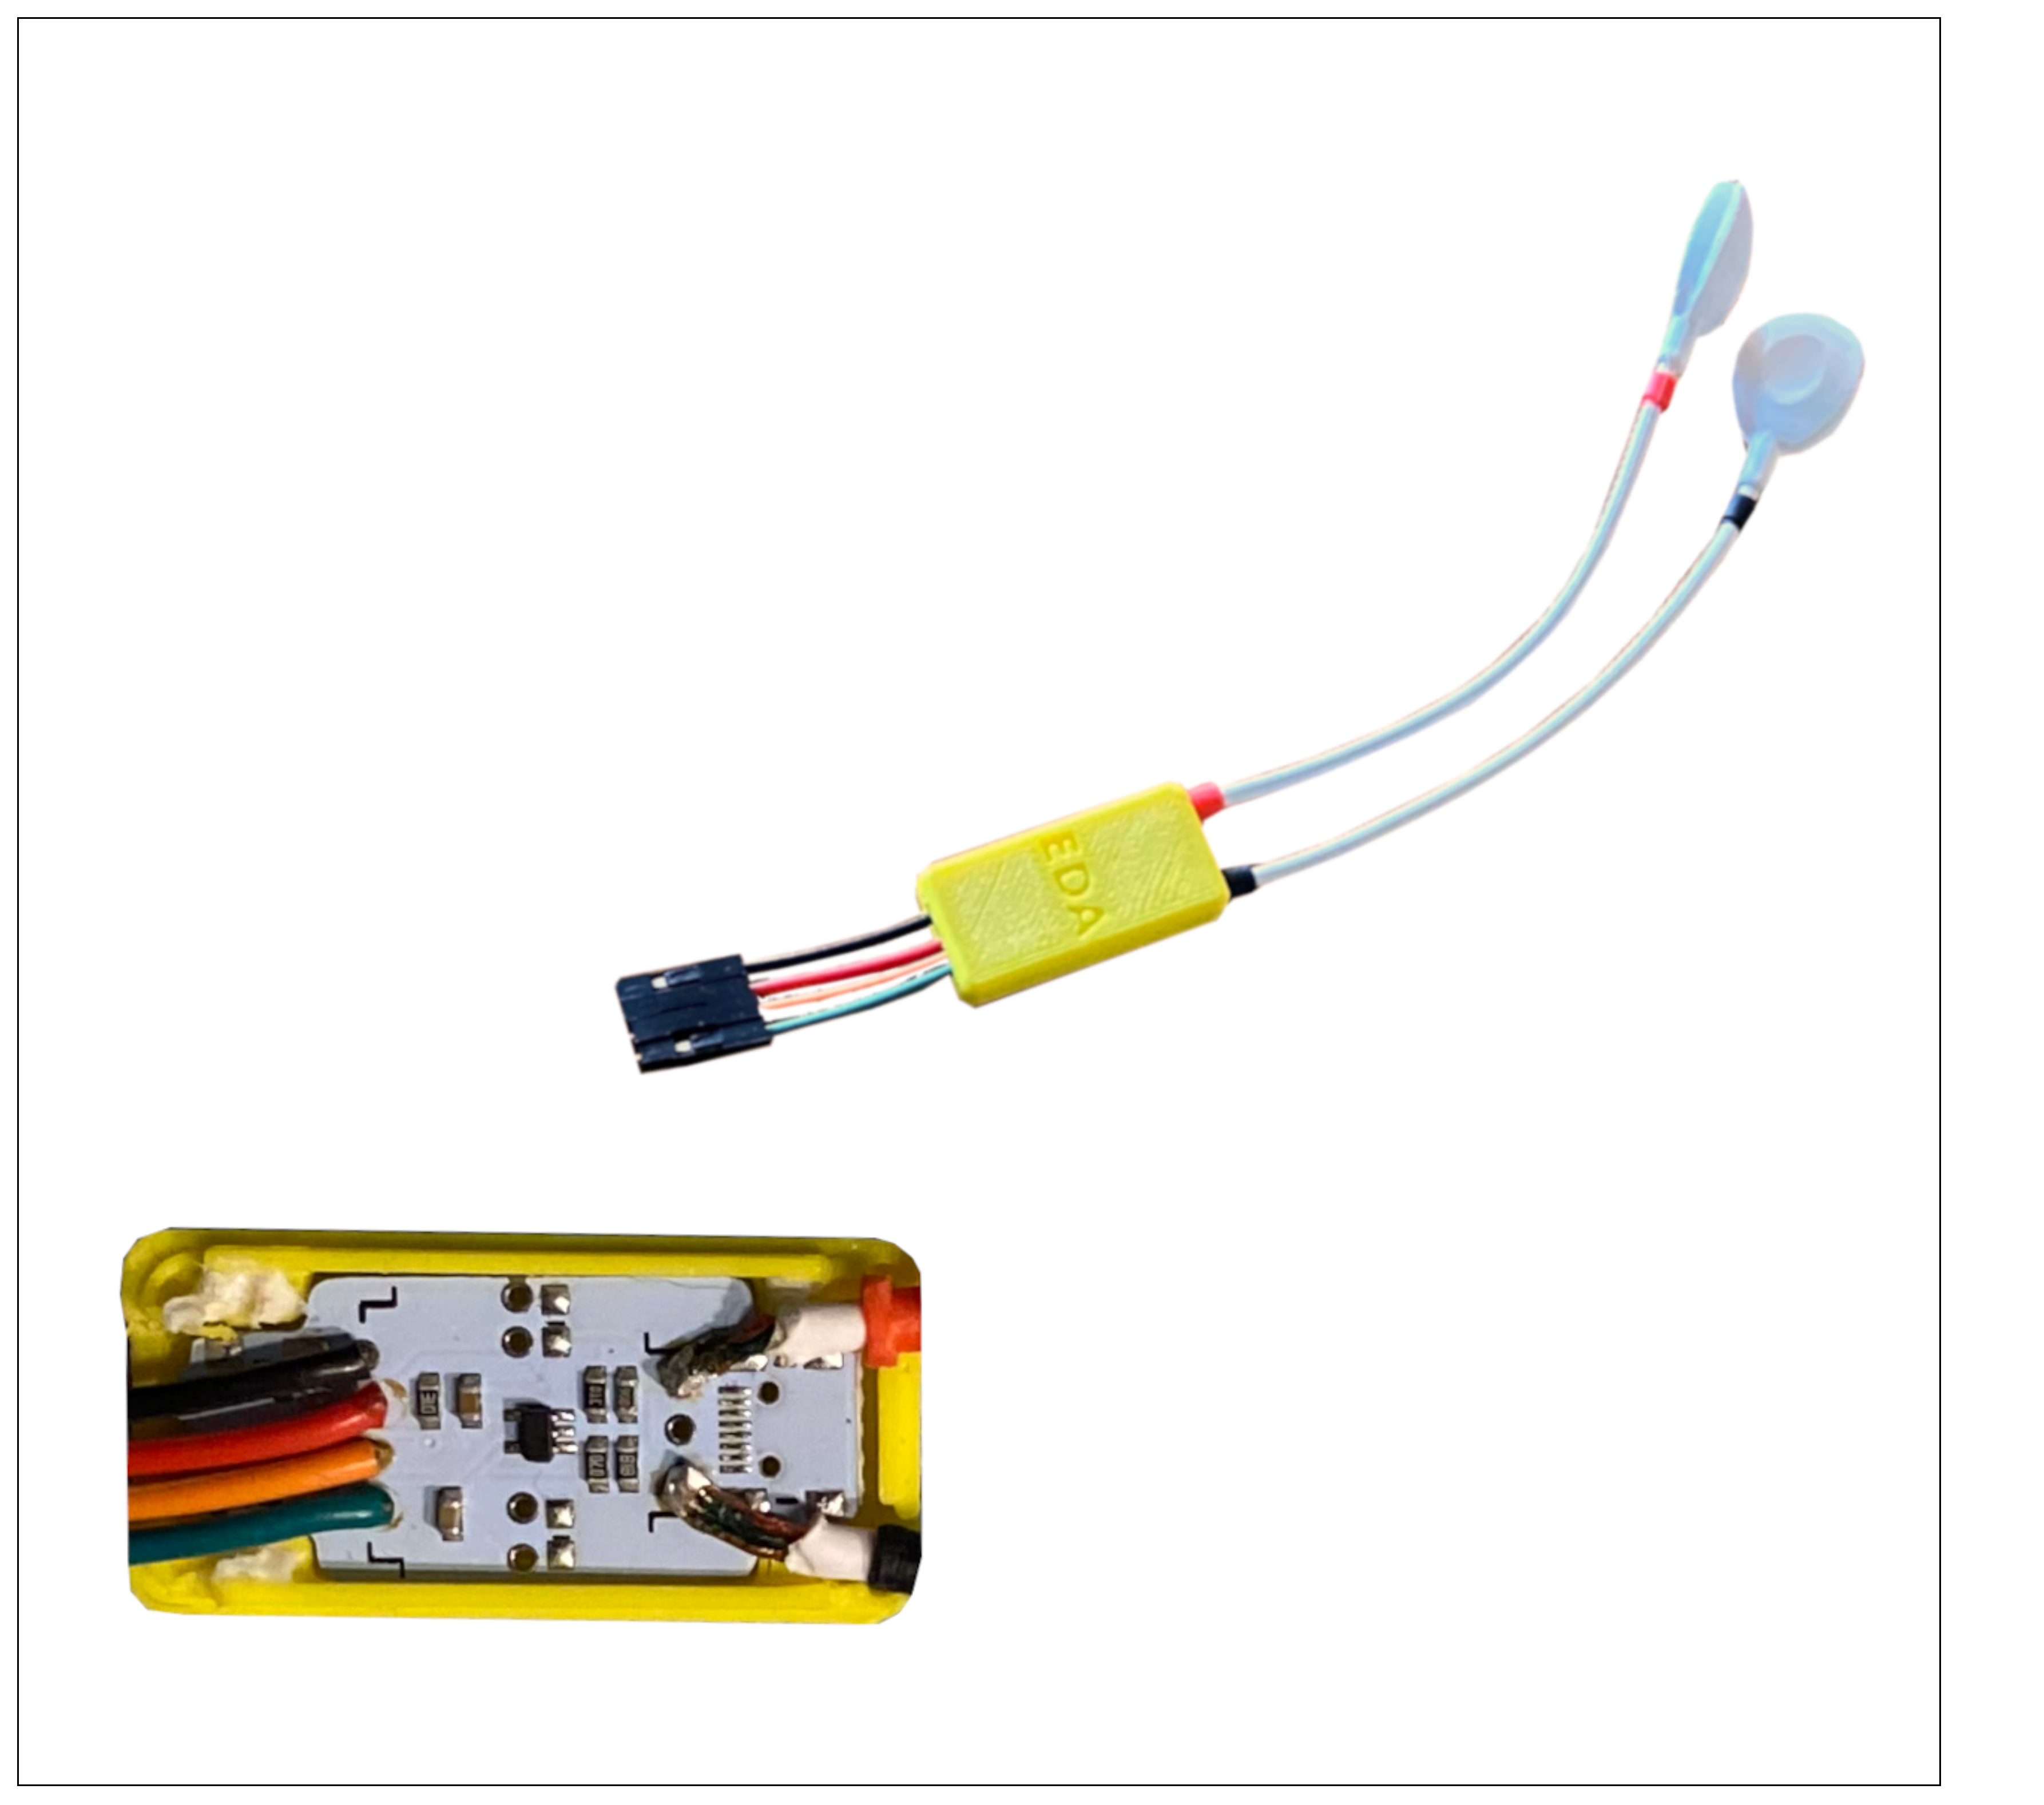
\includegraphics[width=10cm]{./images/full-sensor-view.drawio.png}
    \caption{End result after applying the modifications described}
    \label{fig:full-sensor-configuration}
\end{figure}

\begin{figure}
    \centering
    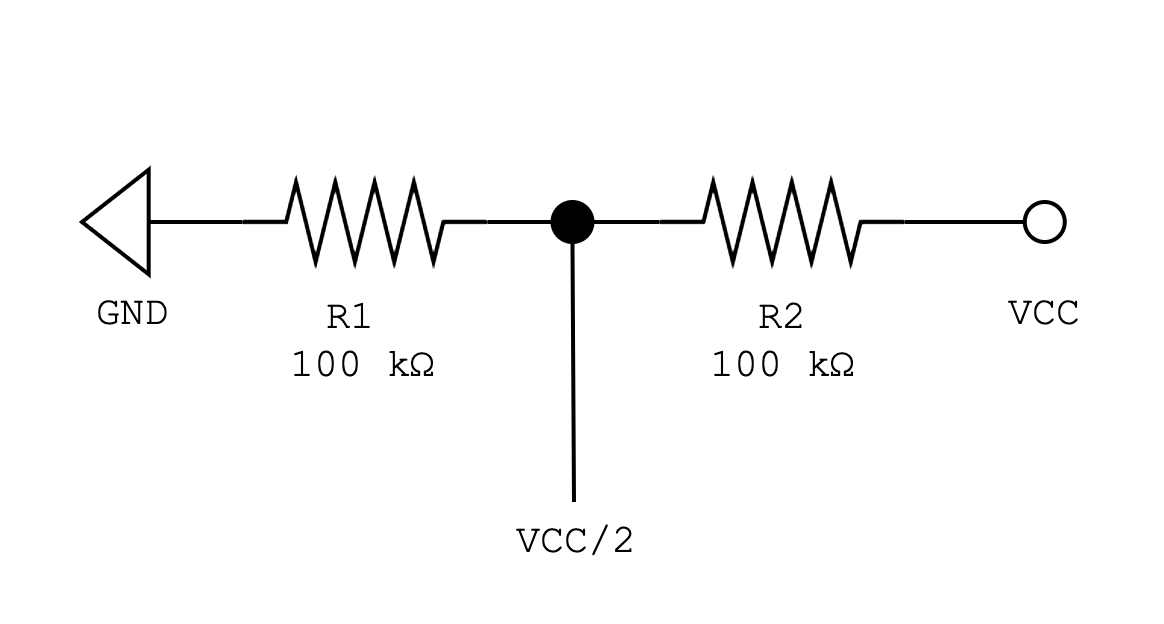
\includegraphics[width=11cm]{./images/midpoint-resistor.drawio.png}
    \caption{Mid-point resistor implemented for the \texttt{VCC/2} pin}
    \label{fig:voltage-divider-schema}
\end{figure}

\begin{figure}
    \begingroup
    \Large
    \begin{equation}
    EDA(\mu S) = \frac{\frac{ADC}{2^n} \cdot VCC}{0.132}
    \end{equation}
    \caption{Transfer function employed for the BITalino EDA sensor}
    \label{fig:bitalino-transfer-function}
    \endgroup
\end{figure}

\pagebreak

\section{Developing a firmware based on the Arduino Framework}\label{sec:firmware}

After applying the necessary changes to the EDA sensor, a research was conducted in order to select an optimal microcontroller upon the following principles: 

\begin{itemize}
    \item Providing a cost-effective solution
    \item Dimensions geared towards high mobility contexts such as fall detection experimentations
    \item Ability to control the system remotely
    \item Limited battery consumption
\end{itemize}

\subsection{Hardware Employed}\label{sec:hardware-employed}

In accordance with the above-stated requirements, a unit based on the well-known \textbf{ESP8266} was employed. The latter consisted, more specifically, of the \textbf{D1 Mini by Wemos} board, which provides easy access to a multitude of functionalities maintaining limited dimensions.

\subsubsection{An overview of the ESP8266}\label{sec:esp8266}

% cite https://en.wikipedia.org/wiki/ESP8266

The ESP8266 consists of an inexpensive 32-bit microcontroller based on the L106 RISC microprocessor that is produced by Espressif Systems. It is widely known and employed in IoT contexts because of its limited dimensions and its native implementation of a full TCP/IP stack, allowing the development of networking-based applications without requiring additional hardware \cite{esp8266}.

Furthermore, the unit exposes 17 GPIO pins which provide a 10-bit resolution analog input and external hardware interfacing through the following protocols:

\begin{itemize}
    \item UART (which allows asynchronous serial communication)
    \item Serial Peripheral Interface (which allows synchronous serial communication)
    \item I$^2$C
    \item I$^2$S
    \item IEEE 802.11 b/g/n
\end{itemize}

Moreover, the ESP8266 offers a capacious flash memory of various Megabytes according to the chosen version and configuration. The latter features allows the indexing of apposite file systems in order to provide persistent memory over restarts. The unit does, though, not provide compatibility with the Bluetooth Low Energy protocol stack (which is a feature that was implemented for the following model, the ESP32).

Additionally, besides Espressif provides its own Software Development Kit (SDK), a multitude of open-source SDKs has been developed over the years. Among all of them, the \textbf{Arduino Framework} stands out because of its accessibility and thanks to the multitude of libraries available. 

\subsubsection{Wemos D1 Mini}\label{subsubsec:d1mini}

For the purposes of this research, a ready-made ESP8266 based board named "Wemos D1 Mini" was employed. The latter provides 16 pins divided into:

\begin{itemize}
    \item 11 digital I/O
    \item 1 analog I/O
    \item 1 RST pin configured for control and reset functions
    \item A single pin for 5V input voltage
    \item A single pin for 3.3V input voltage, which cannot be used together with the 5V one
\end{itemize}

Additionally, the board provides a \textbf{Micro-USB} port which can provide input voltage (substituting the role of the 5V input pin) and data transfer. This allows user to flash compiled binaries to the microcontroller memory in order to execute them. Moreover, since the ESP8266 requires a constant 3.3V input current, the D1 Mini implements a \textbf{voltage regulator} in order to provide the correct internal current, even when the power source provides a voltage above the limit (such as when the unit is powered by a USB cable).

In terms of power consumption, the D1 Mini has a constant drain of 85 mA (which can be reduced drastically when the "Deep Sleep" mode is enabled) and reaches a peak corresponding to 800 mA when powered on.

The figure \ref{fig:d1mini} reports a picture of the D1 Mini unit employed for the experimentation, on which all the pins have been soldered in order to facilitate the test activity by using a breadboard.

\begin{figure}[h]
    \centering
    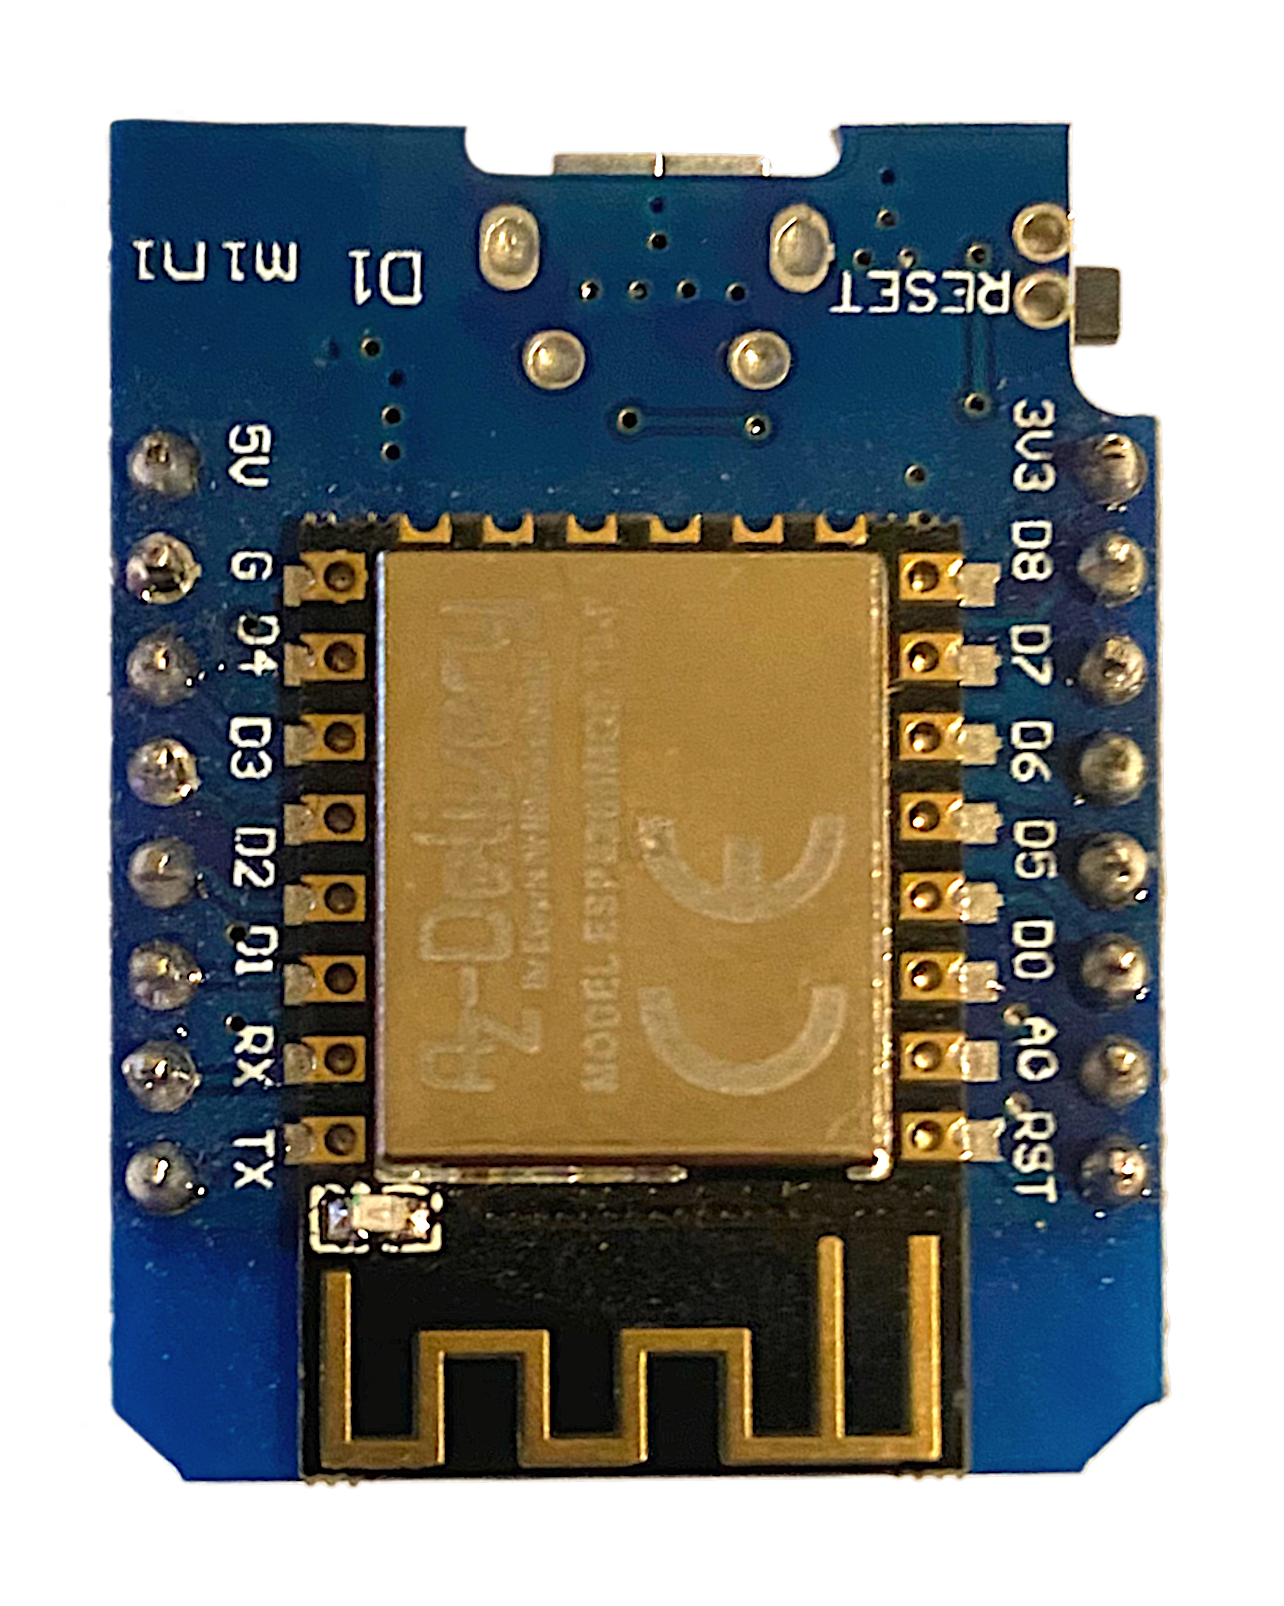
\includegraphics[width=5cm]{./images/d1mini.png}
    \caption{The D1 Mini module employed for the experimentation}
    \label{fig:d1mini}
\end{figure}

\subsubsection{Connection with the BITalino EDA sensor}\label{subsubsec:d1mini}

The modifications applied to the BITalino unit (described in \ref{subsec:bitalno-modifications}) allowed a seamless connection between the D1 Mini and the EDA sensor. The latter was, in fact, directly powered by the microcontroller and connected to its 10-bit resolution analog input. The whole system was, then, powered by a 3.7V-1200mAh Lipo battery. A diagram representing the final circuit is presented in figure \ref{fig:circuit-diagram}

\begin{figure}[h]
    \centering
    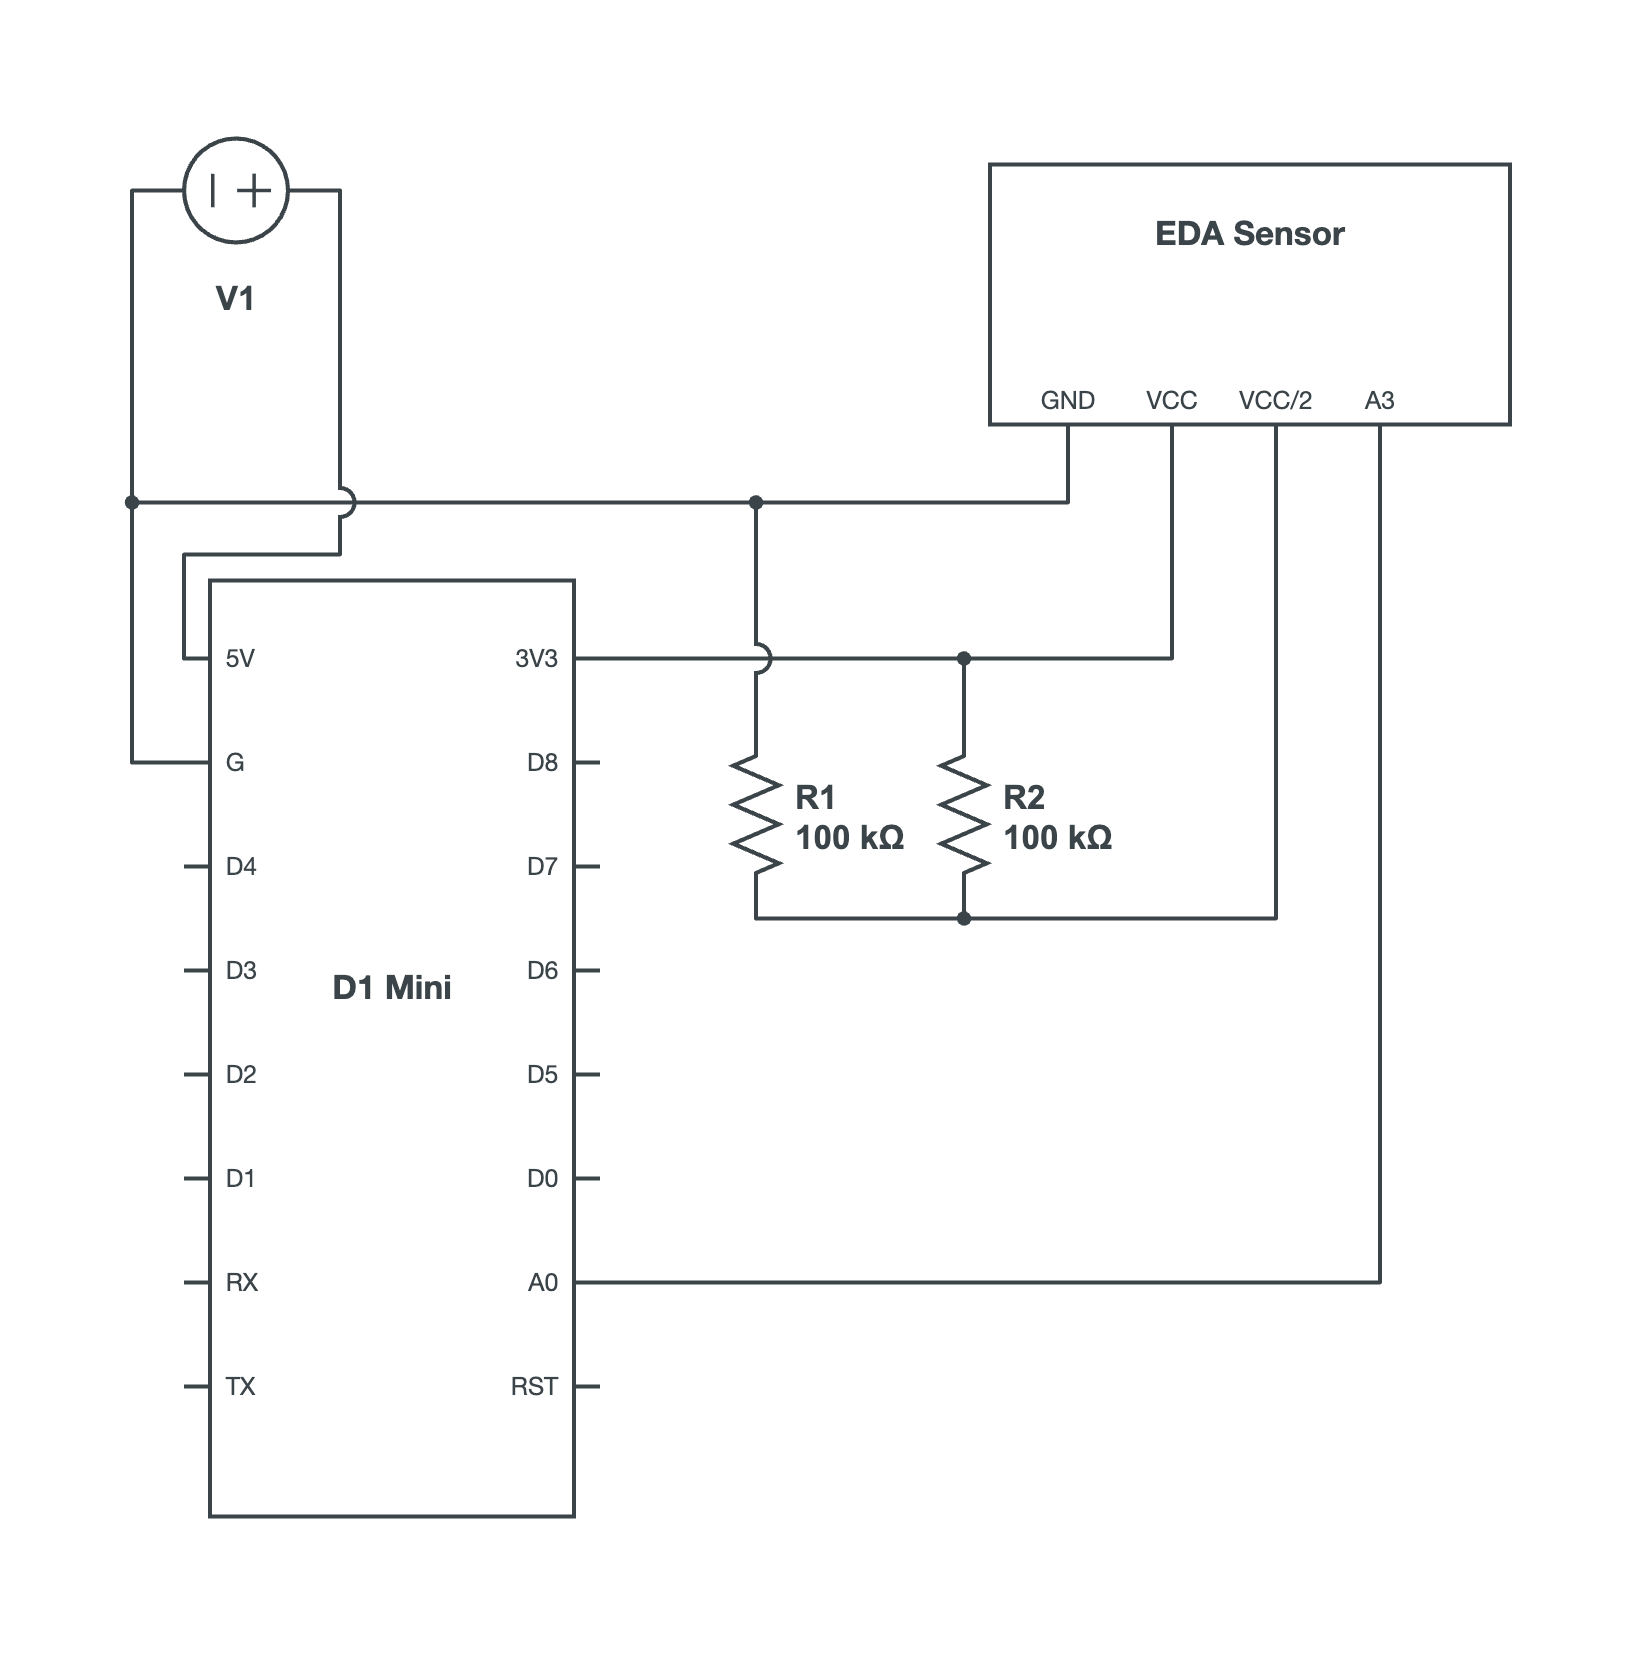
\includegraphics[width=10cm]{./images/circuit-diagram.png}
    \caption{Circuit diagram}
    \label{fig:circuit-diagram}
\end{figure}

The result obtained was finally soldered on a \textbf{matrix board} and packed inside an arm pocket in order to provide protection against the impacts and shocks that a fall may cause.  

\subsection{Firmware Implementation}\label{subsec:firmware-implementation}

As stated previously, the firmware implemented in order to acquire EDA data from the sensor was based on the \textbf{Arduino Framework}, which is at present completely compatible with ESP8266 boards. The latter provides great flexibility and allows easy development for embedded devices. 

The main requirements for the system were the followings:

\begin{itemize}
    \item A functionality that allows the end-user to start each measurement
    \item A functionality that allows to retrieve the measured data
    \item Being able to read data with a sufficiently high sample rate in accordance with the Nyquist Theorem, as stated in \ref{subsec:eda-signal-properties}
\end{itemize}

%IPAddress    apIP(10, 10, 10, 1);                               // Private network address: local & gateway
%
%
%<...>
%void setup() {
%  WiFi.mode(WIFI_AP_STA);
%  WiFi.softAPConfig(apIP, apIP, IPAddress(255, 255, 255, 0));   // subnet FF FF FF 00
%  WiFi.softAP("TardisTime");

In order to address the aforementioned requirements, the device was configured as a \textbf{Soft Access Point} exposing a \textbf{RESTful WebServer} which provides a series of endpoints according to the functionalities required to start each measurement and retrieve the collected data. The EDA activity was sampled at 100 Hz and retrieved from the sensor by employing a logic based on \textbf{Interrupt Service Routines}. The obtained data was, then, buffered and saved on a minimal file system indexed on the flash memory of the microcontroller.

\subsubsection{Libraries Employed}\label{subsubsec:libraries-employed}

In order to exploit the various functionalities required, two additional libraries were included besides the Standard Library that composes the Arduino Framework:

\begin{itemize}
    \item \textbf{LittleFS}
    \item \textbf{ESP8266TimerInterrupt}
\end{itemize}

\textbf{LittleFS} is a library that provides primitives to index and access a file system from the EEPROM (Electrically Erasable Programmable Read-Only Memory) of micro-controllers. It is designed in order to work with limited amounts of storage, providing power-loss resilience and dynamic wear leveling \cite{littlefs}. The latter results fundamental in order to prolong the memory life, which would otherwise be extremely limited in case of micro-controllers. This is made possible be providing a hash-map data structure that maintains a reference for each logical block address that composes the memory space and its current status, in order to select blocks with the lowest erase count for the following write. Furthermore, the library provides functionalities for buffered reading and writing. It was employed in order to gradually save the data retrieved from the EDA sensor in a binary file.

\vspace{8mm}

\textbf{ESP8266TimerInterrupt} enables, instead, the definition of Interrupt Service Routines based on Hardware Timers on ESP8266-based boards \cite{esp8266timerinterrupt}. The latter were employed in order to provide a 100 Hz constant readout from the EDA sensor, by defining a timer that triggers an ISR (which reads data from the sensor and buffers the result) every 10ms.

\vspace{8mm}
A
The firmware was developed in \texttt{C++} using PlatformIO, an open-source framework licensed under the Apache 2.0 license \cite{platformio} which provides several functionalities for embedded development, including scripts for flashing programs to the devices and debug them.

\subsubsection{Program Structure}\label{subsubsec:program-structure}

As required by the Arduino Framework, then program relies on a \mintinline{cpp}{void setup()} function which is executed once everytime the device is started and a \mintinline{cpp}{void loop()} which is, then, executed repeatedly. After including the required libraries, two macro directives were specified in order to indicate the analog pin used for the sensor reading and the sample rate (which is specified in Hz).

\begin{minted}{cpp}
#define EDAPIN A0
#define EDA_SAMPLE_RATE 100
\end{minted}

The main variables and handlers were, then, defined with a global scope. This was performed in order to provide access to:

\begin{itemize}
    \item The \textbf{ESP8266WebServer} handler
    \item The \textbf{ESP8266Timer} handler
    \item The current file descriptor provided by \textbf{LittleFS}
    \item Synchronization flags, declared as \mintinline{cpp}{volatile} when accessed by the Interrupt Service Routine
\end{itemize}

\begin{minted}[frame=single,framesep=10pt]{cpp}
volatile int measurementDuration = 60;
volatile bool measuring = false;
volatile int measurementStart;

IPAddress localIP(192,168,4,22);
IPAddress gateway(192,168,4,9);
IPAddress subnet(255,255,255,0);
ESP8266WebServer server(80);

ESP8266Timer ITimer;

char paramsBuffer[100];
byte payload[12];
File file;
\end{minted}

The setup function configures the WebServer and the Hardware Timer, other than specifying the role of the \texttt{A0} pin. More specifically, the \texttt{/}, \texttt{/start} and \texttt{/retrieve} endpoints are defined in order to respectively acquire informations about the device status, start a measurement for the specified duration and retrieve the previously stored data.

\begin{minted}[frame=single,framesep=10pt]{cpp}
void setup() {
    pinMode(A0, INPUT);

    WiFi.softAPConfig(localIP, gateway, subnet);
    
    if (!WiFi.softAP("eda-measurement", NULL, 1, 0, 1)) {
        Serial.println("Unable to run as Soft Access Point");
        while(1);
    }

    if (!LittleFS.begin()) {
        Serial.println("Unable to run as Soft Access Point");
        while(1);
    }

    ITimer.attachInterrupt(EDA_SAMPLE_RATE, ISRHandler);

    server.on("/", HTTP_GET, info);
    server.on("/start", HTTP_POST, start);
    server.on("/retrieve", HTTP_GET, retrieve);
    server.begin();
}
\end{minted}

More specifically, the \texttt{/start} endpoint starts a measurement for a specified duration and saves the data on a binary file whose name is also specified as a request parameter.

\begin{minted}[frame=single,framesep=10pt]{cpp}
bool initializeNewFile(char *name) {
    return (file = LittleFS.open(name, "w"));
}

void startMeasurement(int durationInSeconds) {
    measurementDuration = durationInSeconds;
    measurementStart = millis();
    measuring = true;
}

void start() {
    const char *args = server.arg("plain").c_str();

    strcpy(paramsBuffer, args);
    char *filename = strtok(paramsBuffer, "|");
    int duration = atoi(strtok(NULL, "|"));

    if (initializeNewFile(filename)) {
        startMeasurement(duration);
        server.send(200, "plain/text", "Starting measurement");
    } else {
        server.send(500, "plain/text", "Unable to initialize a new reading");
    }
}
\end{minted}

The interrupt service routine performs an \mintinline{cpp}{analogRead()} on the EDA sensor pin. Subsequently, the value read from the sensor is combined, together with the one returned by \mintinline{cpp}{millis()}, in a 12-byte payload (using bit-wise operators). The latter is, then, written to the memory as binary data. This is performed by the two following subroutines.

%pagebreak % added to move the whole code block to a new page since the previous one is almost ending

\begin{minted}[frame=single,framesep=10pt]{cpp}

void writeNewDataLine(int sample, long timestamp) {
    payload[0] = (sample >> 24) & 0xFF;
    payload[1] = (sample >> 16) & 0xFF;
    payload[2] = (sample >> 8) & 0xFF;
    payload[3] = sample & 0xFF;  

    payload[4] = (timestamp >> 56) & 0xFF;
    payload[5] = (timestamp >> 48) & 0xFF;
    payload[6] = (timestamp >> 40) & 0xFF;
    payload[7] = (timestamp >> 32) & 0xFF;
    payload[8] = (timestamp >> 24) & 0xFF;
    payload[9] = (timestamp >> 16) & 0xFF;
    payload[10] = (timestamp >> 8) & 0xFF;
    payload[11] = timestamp & 0xFF;

    file.write(payload, 12);
}

void IRAM_ATTR ISRHandler(void) {
    if (measuring) {
        writeNewDataLine(analogRead(EDAPIN), millis());
    }
}
\end{minted}

It is important to note that \mintinline{cpp}{millis()} returns the number of milliseconds elapsed since the microcontroller was powered. Its value was acquired in order to determine the number of milliseconds elapsed between each measurement.

The following subroutine was, instead, defined in order to stop the measurement and save the binary data to the memory storage:

%pagebreak

\begin{minted}[frame=single,framesep=10pt]{cpp}

bool closeFile() {
    if (file) {
        file.close();
        return true;
    }
    return false;
}

bool stop() {
    if (measuring) {
        measuring = false;
        closeFile();
        return true;
    }
    return false;
}
\end{minted}

The \texttt{/retrieve} endpoint was, then, defined in order to send the required binary data as an application/octet-stream mimetype. Once completely streamed to the client, the file is subsequently removed from the memory storage.

\begin{minted}[frame=single,framesep=10pt]{cpp}
void retrieve() {
    String filename = server.arg("plain");
    file = LittleFS.open(filename, "r");

    if (file) {
        server.sendHeader("Content-Type", "text/text");
        server.sendHeader("Content-Disposition", 
                          "attachment; filename=" + filename);
        server.sendHeader("Connection", "close");
        server.streamFile(file, "application/octet-stream");
        file.close();
        LittleFS.remove(filename);
    } else {
        server.send(200, "plain/text", 
                    "Unable to retrieve measurement from memory");
    }
}
\end{minted}

Finally, the \mintinline{cpp}{void loop()} function was configured in order to poll incoming HTTP requests when no measurement is happening or, otherwise, determine when to stop the currently running measurement. This was done with the aim of preventing HTTP requests during a measurement, since both the Wi-Fi antenna and the EDA sensor rely on the same (and only) analog input of the microcontroller.

\begin{minted}[frame=single,framesep=10pt]{cpp}
void loop() {
    if (!measuring) {
        server.handleClient();
    } else {
        const long currentMillis = millis();
        if (currentMillis - measurementStart > measurementDuration * 1000 ) {
            stop();
        }
    }
}
\end{minted}

\pagebreak

\section{Data Collection}\label{sec:data-collection}

% TODO ALTFRAILTY

The device was tested during a session of the \textbf{WP8 ALT-FRAILTY} dataset acquisition. More specifically, the falls reported in table \ref{toc:bitalino-falls} were performed by a 22 years old male volunteer wearing the device on his non-dominant arm.

\vspace{7mm}

\begin{table}[H]
\centering
\begin{tabular}{ll}
    \hline
    Name            &  Description           \\
    \hline
    Rolling         & Falling forward from a chair, landing on the knees \\
    Left Shoulder   & Standing and subsequently falling on the left shoulder \\
    Right Shoulder  & Standing and subsequently falling on the right shoulder \\
    Sidewards       & Standing and subsequently falling sidewards directly on the ground \\
    Bed             & Falling while getting up from the bed \\
    \hline
\end{tabular}
\caption{Falls performed during the first experimentation}
\label{toc:bitalino-falls}
\end{table}

